
\section{Overview}

The restricted arrays functionality is designed to provide users with
further options for how data is distributed among processors by allowing
them to reduce the total number of processors that actually have data
and also by allowing users to remap which data blocks go to which
processors. There are two calls that allow users to create restricted
arrays; both must be used with the new interface for creating arrays.
This requires that users must first create an array handle using the
\texttt{ga\_create\_handle} call and then apply properties to the
handle using different ga\_set calls. The two calls that allow users
to create restricted arrays are \texttt{ga\_set\_restricted} and \texttt{ga\_set\_restricted\_range}.
The first call is more general, the second is a convenience call that
allows users to create restricted arrays on a contiguous set of processors. 

Both calls allow users to restrict the data in a global array to a
subset of available processors. The set ga\_set\_restricted call has
two arguments, \texttt{nproc}, and an array \texttt{list} of size
\texttt{nproc}. Nproc represents the number of processors that are
supposed to contain data and list is an array of the processor IDs
that contain data. For the array shown in Figure \ref{cap:GA-36Processors},
the problem is run on 36 processors but for nproc=4 and list={[}8,9,15,21{]}
only the processors shown in the figure will have data. The array
will be decomposed assuming that it is distributed amongst only 4
processors so it will be broken up using either a 2x2, 1x4, or 4x1
decomposition. The block that would normally be mapped to process
0 in a 4 processor decomposition will go to process 8, the data that
would map to process 1 will go to process 9, etc. This functionality
can be used to create global arrays that have data limited to a small
set of processors but which are visible to all processors. 

%
\begin{figure}
\begin{centering}
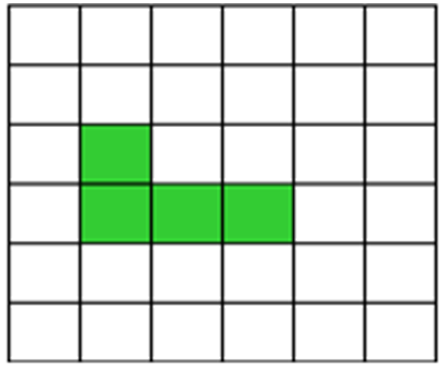
\includegraphics[width=3in]{GAon36Processors}
\par\end{centering}

\caption{\label{cap:GA-36Processors}A global array distributed on 36 processors.
If nproc=4 and list = {[}8,9,15,21{]} then only the shaded processor
will contain data. The array will be decomposed into 4 blocks. }

\end{figure}


The restricted array capability can also be used to alter the default
distribution of data. This is ordinarily done in a column major way
on the processor grid so that a global array created on 16 processors
that has been decomposed into a 4x4 grid of data blocks would have
data mapped out as shown in Figure \ref{fig:GA-16-Standard-data-distribution}.
The first column of blocks is assigned to processes 0-3, the second
to processes 4-7, etc. 

%
\begin{figure}
\begin{centering}
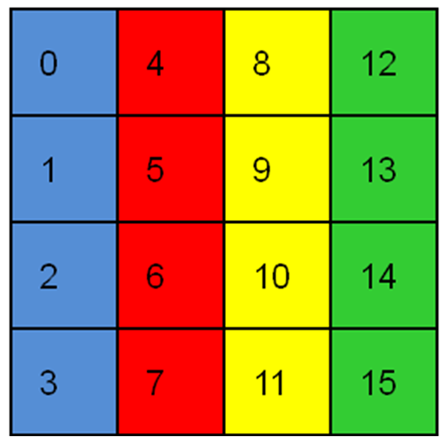
\includegraphics[width=3in]{GAon16Processors}
\par\end{centering}

\caption{\label{fig:GA-16-Standard-data-distribution}Standard data distribution
for a global array created on 16 processors and decomposed into a
4x4 grid of data blocks. }



\end{figure}


Figure \ref{fig:GA-16-An-alternative-distribution} shows an alternative
distribution that could be achieved using restricted arrays and setting
the list array to {[}0,1,4,5,2,3,6,7,8,9,12,13,10,11,14,15{]}. This
distribution might but useful for reducing intranode communication
for multiprocessor nodes 

%
\begin{figure}
\begin{centering}
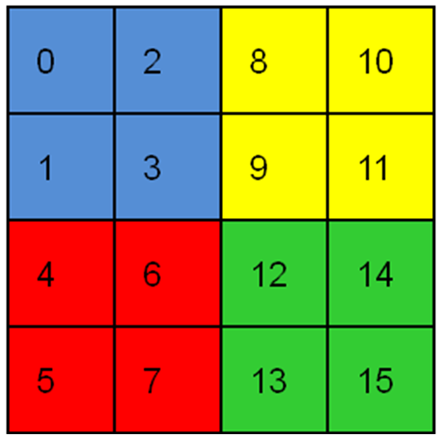
\includegraphics[width=3in]{GAon16ProcessorsAlternative}
\par\end{centering}

\caption{\label{fig:GA-16-An-alternative-distribution}An alternative distribution
that could be achieved using restricted arrays. An array on 16 processors
decomposed into a 4x4 grid of data blocks. }



\end{figure}



\section{Restricted Arrays Operations}
\begin{lyxcode}
\textcolor{blue}{Fortran}~subroutine~ga\_set\_restricted(g\_a,~list,~nproc)~

\textcolor{blue}{C~}~~~~~~void~GA\_Set\_restricted(int~g\_a,~int~list{[}{]},~int~nproc)~

\textcolor{blue}{C++}~~~~~GA::GlobalArray::setRestricted(int~list{[}{]},~int~nproc)~const
\end{lyxcode}
This subroutine restricts data in the global array \texttt{g\_a} to
only the \texttt{nproc} processors listed in the array list. The value
of \texttt{nproc} must be less than or equal to the number of available
processors. If this call is used in conjunction with \texttt{ga\_set\_irreg\_distr},
then the decomposition in the \texttt{ga\_set\_irreg\_distr} call
must be done assuming the number of processors used in the \texttt{ga\_set\_restricted}
call. The data that would ordinarily get mapped to process 0 in an
\texttt{nproc} distribution will get mapped to the processor in \texttt{list{[}0{]}},
the data that would be mapped to process 1 will get mapped to \texttt{list{[}1{]}},
etc. This can be used to restructure the data layout in a global array
even if the value of \texttt{nproc} equals the total number of processors
available. 
\begin{lyxcode}
\textcolor{blue}{Fortran}~subroutine~ga\_set\_restricted\_range(g\_a,~list,~nproc)~

\textcolor{blue}{C}~~~~~~~void~GA\_Set\_restricted\_range(int~g\_a,~int~lo\_proc,~

~~~~~~~~~~~~~~~~~~~~~~~~~~~~~~~~~~~~~int~hi\_proc)~

\textcolor{blue}{C++~}~~~~GA::GlobalArray::setRestrictedRange(int~lo\_proc,~

~~~~~~~~~~~~~~~~~~~~~~~~~~~~~~~~~~~~~~~~~~~~int~hi\_proc)~const
\end{lyxcode}
This subroutine restricts data in the global array \texttt{g\_a} to
the processors beginning with\texttt{ lo\_proc} and ending with \texttt{hi\_proc}.
Both \texttt{lo\_proc} and \texttt{hi\_proc} must be less than or
equal to the total number of processors available minus one (e.g.,
in the range \texttt{{[}0,N-1{]}} where N is the total number of processors)
and \texttt{lo\_proc} must be less than or equal to \texttt{hi\_proc}.
If \texttt{lo\_proc=0} and \texttt{hi\_proc=N-1} then this command
has no effect on the data distribution. This call is equivalent to
using the \texttt{ga\_set\_restricted} call where \texttt{nprocs =
hi\_proc-lo\_proc+1} and the array \texttt{list} contains the processors
\texttt{{[}lo\_proc, hi\_proc{]}} in consecutive order. 
